\chapter{Hybrid Ray tracer}
\label{chapter:hybrid}
%----------------------------------------------------------------------------------------
%	HYBRID RAY TRACER	
%----------------------------------------------------------------------------------------
\section{Shortcomings of the exponential ice model}
As mentioned in section \ref{section:Ice Model}, complex ice models will be
necessary moving forward as the exponential ice model fails to fit the density
curve.  The software for radio wave propagation through ice the RNO-G team
chose is radiopropa\cite{Winchen_2019}, but due to the way it works you'll have
to know the start point, the end point and the launch angle of your ray to work
out the path. This isn't difficult for the analytic model as it's exactly
solvable but for a general ice model you'll somehow have to find where to
\textit{shoot} the ray. An algorithm was developed to work out the path the
rays would trace out in more complex ice models called the \textit{iterative
ray tracer} \cite{2022icrc.confE1027O}, which was discussed in section
\ref{sec:Iterative}. The way this algorithm works is however a sub-optimal
solution in python as an optimalisation library will generally work faster and
more accurate, work had been done on trying to implement such an algorithm
deemed the "minimizer" but this attempt failed.  As we saw this work the idea
came to mind to combine the iterative ray tracer and the code using the
optimization libraries. This way we built the algorithm which will be discussed in
this chapter: The hybrid ray tracer, in the source code called the "hybrid
minimizer" which can be found
\href{https://github.com/arthuradriaens-code/NuRadioMC.git}{here} under the
radiopropa/hybrid\_minimizer branch.

It succeeds in more rapidly finding the path from the event to the detector, is
more accurate and also arrives closer to the detector as the final result is
not limited by the final drawn sphere size but by a given tolerence making it
useful for simulations in which high time and space precision is needed like
plane wave reconstruction, which we'll do in the next chapter.

\section{How it works}
The hybrid minimizer can be seen as an extension of the iterative raytracer as
it starts out the same way: Say our source of radiation is at position
$\mathbf{X}_1$ and our detector is located at position $\mathbf{X}_2$, we start
by defining the vector $\mathbf{v} = \mathbf{X}_2 - \mathbf{X}_1$, then we
clone it as a new vector $\mathbf{u}$ and set it's z coordinate to 0, making it a normal
vector of a plane parallel to the z direction in the lateral direction of the detector. 
We now want to constrain the search to where solutions are actually possible, 
looking at figure \ref{fig:PathIllu}
we see that no solutions below the direct path are possible as there would need
to be upwards reflection, so we convert our vector $\mathbf{v}$ representing
the path from the source to the detector to spherical coordinates, giving us a
polar angle (zenith angle) "theta-direct". With this we know that from the source
the ray should propagate with an initial zenith angle lying within the angle interval
0° to theta-direct° $:= \Omega$ ($\theta \in ]0,\Omega]$).

Next we need to define our "observers", if you shoot a ray with the radiopropa
module from a certain point at a certain angle the ray path will get simulated
until it interacts with this "observer".  Ideally we would like to a priori
know where to shoot our ray and have the detector be an infinitesimally small
observer in our simulation, but as we'll be working with general ice models
this can't be done.

The algorithm of finding the possible paths is then as follows: We define a
spherical observer at the location of the detector, with a radius of fair
size\footnote{We'll get back to how this "fair size" gets chosen}.  We place an observer plane directly
behind the detector with normal vector $\mathbf{u}$ (as no rays can propagate
back after passing the detector) and an observer above the surface (as no rays
could make it back after escaping the ice) our full setup is then what's
illustrated in figure \ref{fig:Illustration of hybrid algorithm}

\begin{figure}
  \centering
  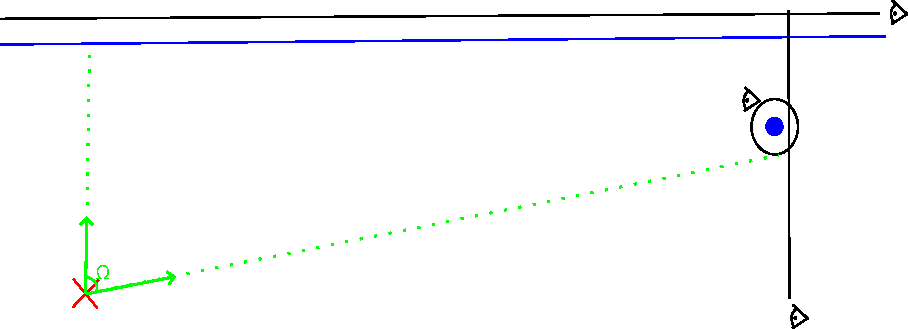
\includegraphics[width=0.7\textwidth]{algoillu.pdf}
  \caption{Illustration of the workings of the hybrid algorithm}
  \label{fig:Illustration of hybrid algorithm}
\end{figure}

Here the red cross is the radio source, the blue horizontal line is the ice-air
boundary surface, the blue dot to the right is the detector and the green
$\Omega$ indicates the range over which solutions to the problem are possible.

We start off by just iteratively guessing: given a certain angle stepsize
$\Delta \theta$ shoot rays at the angles $\{0,\Delta \theta, 2\Delta
\theta,...,\Omega\}$ And see which ones get detected at the sphere around the
detector, this process is illustrated in figure \ref{figure:First step hybrid}.
\begin{figure}
	\centering
	\copyrightbox[r]{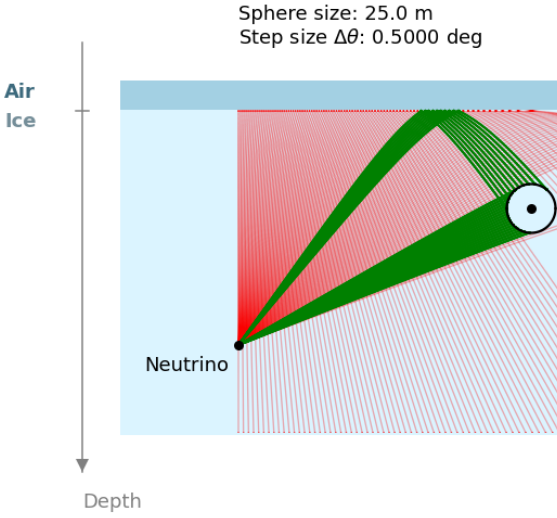
\includegraphics[width=0.5\textwidth]{begin_explanation.png}}{\textcopyright Effects of firn ice models on radio neutrino simulations using a RadioPropa ray tracer by B. Oeyen et. al}
	\caption{First step of the hybrid ray tracer}
	\label{figure:First step hybrid}
\end{figure}

If 2 distinct launch regions are found, say in the regions $[\theta_1,\theta_2]$ and $[\theta_3,\theta_4]$ the
rays end up on the sphere (drawn in green), then the so called \textit{minimization}
procedure will start. Using scipy's module optimize.minimize the optimal
solution will be found. First we get rid of the spherical observer and place
the vertical observer \textbf{exactly} at the detector, now to be able to use the
minimize module we'll need a function to minimze, for this reason we first define the
function \textit{delta\_z} as, given a certain launch angle, propagating the ray
onto the vertical observer and returning the
distance from the point where it lands on the plane to the detector, as
illustrated on figure \ref{fig:PrincipleHybridIllu} (i.e it returns the value $\Delta z$).
\begin{figure}
  \centering
  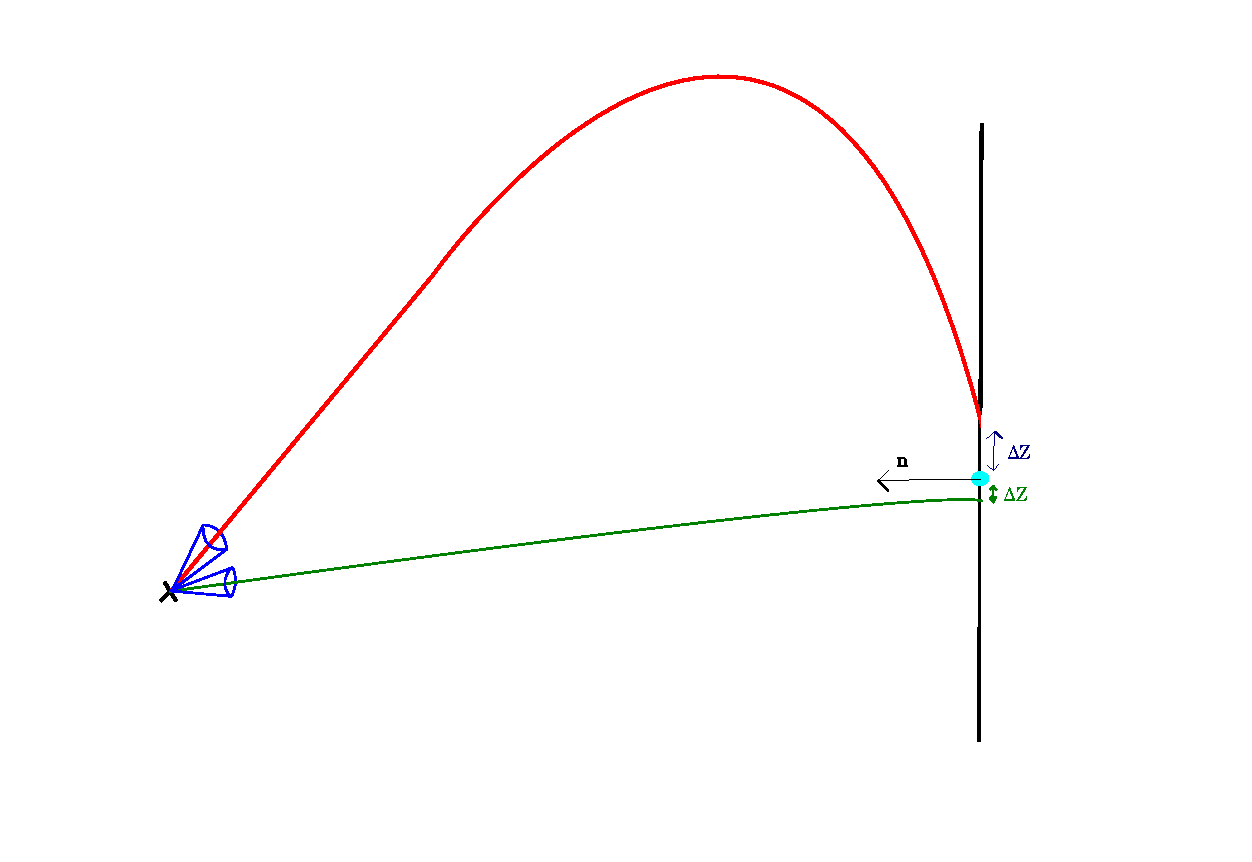
\includegraphics[width=0.5\textwidth]{PrincipleHybridIllu.pdf}
  \caption{Principle behind the minimization in the hybrid ray tracer}
  \label{fig:PrincipleHybridIllu}
\end{figure}
The function we'll minimize is then delta\_z\_squared which just squares the
value which delta\_z returns as we want to do away with negative values (so we
can minimize to $\Delta z=0$). We use the previously found angle boundaries as
the boundaries for this minimization algorithm, meaning that if the 2 zenith
angle intervals $[\theta_1,\theta_2]$ and $[\theta_3,\theta_4]$ were found in
the first step of the algorithm it will first minimize $\Delta z^2$ within the
first angle interval and find it's solution and then within the second angle
interval. With this our algorithm is done, it does have a fail-safe as well for
if the first step, finding the launch regions, doesn't find the 2 launch
regions.  Namely it reverts back to being the iterative ray tracer.

\section{Performance Optimalisation} 
We wish to optimize this algorithm to make
it as fast as possible.  To consistently test the algorithm after every
particular change in a parameter we'll be randomly generating vertex
interaction positions, keeping the detector at the fixed (0,-100) value.  To
this end the numpy random module was used to generate random coördinates, the
considered square (as there is only a z component to the ice model the 3D
problem is cilindrically symmetric and thus essentially only a 2D problem) is
x:0.1km,4km and z:-0.1km,-3km\footnote{This start at 100m depth was to get
around issues concerning events that won't even trigger in a full simulation}.
Every simulated point shown in the following subsections consists of at least
500 random initial positions.  As the speed of the algorithm is computer
dependent the algorithm's speed is always plotted relative to the iterative ray
tracer's speed, simulated with the same coordinates and under equal computer load.

Now we don't want to just achieve higher speed in our algorithm, we also want
to at least have the same accuracy as the iterative ray tracer, if not even better.
To this end we need to check with an "exact solution". There is only one candidate
that fits this role: \textit{the analytic ray tracer}. The plan is thus to use the
exponential ice model as a testing ground for the hybrid ray tracer and solving each
vertex-detector ray tracing problem with both the iterative, analytic and hybrid ray tracer.
After having solved for the \textbf{propagation time}, meaning the time it takes the ray to
propagate from the source to the detector. And the \textbf{arrival zenith angle}, the zenith angle
the ray makes at the detector, for each of the algorithms we can infer the accuracy of a particular
algorithm by how much it differs from the solution found through the analytic ray tracer.
For example, if the hybrid ray tracer finds a particular solution with a propagation time of 
1001ns, the iterative finds one with 1002ns and the analytic one with 1000ns then the hybrid
ray tracer is more accurate than the iterative ray tracer.
\subsection{Length of the normal vector}
\begin{figure}
	\centering
	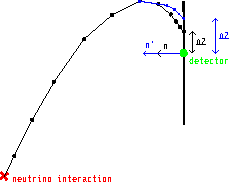
\includegraphics[width=0.7\textwidth]{figures/PrincipleNormIllu.pdf}
	\caption{how normal vector size influences the stepsize}
	\label{fig:normexpl}
\end{figure}
Whilst figuring out what was wrong with the initial \textit{minimizer} we
stumbled on the fact that radiopropa has a little weird quirk.  As visually
explained in figure \ref{fig:normexpl}, the size of the normal vector seems to
influence how big radiopropa's ray tracer's step size is taken close to the
detector.  This thus influences the accuracy and total computational time
taken. The results of varying the length of this normal vector, comparing the
accuracy (in timing and arrival zenith) with the analytic ray tracer and the computational time with the
iterative ray tracer, are shown in figures \ref{fig:norminfl} and
\ref{fig:norminfl2}.  Looking at these figures we can conclude a, what would
normally be rather obvious but is interesting nonetheless, first optimization
conclusion: take the normal vector length to be 1 meter.
We can conclude this as the calculation speed seems to be minimal there (after zooming
in on the graph) and the accurace dropping rapidly after 1 meter.

\begin{figure}
	\centering
	\begin{minipage}{\textwidth}
		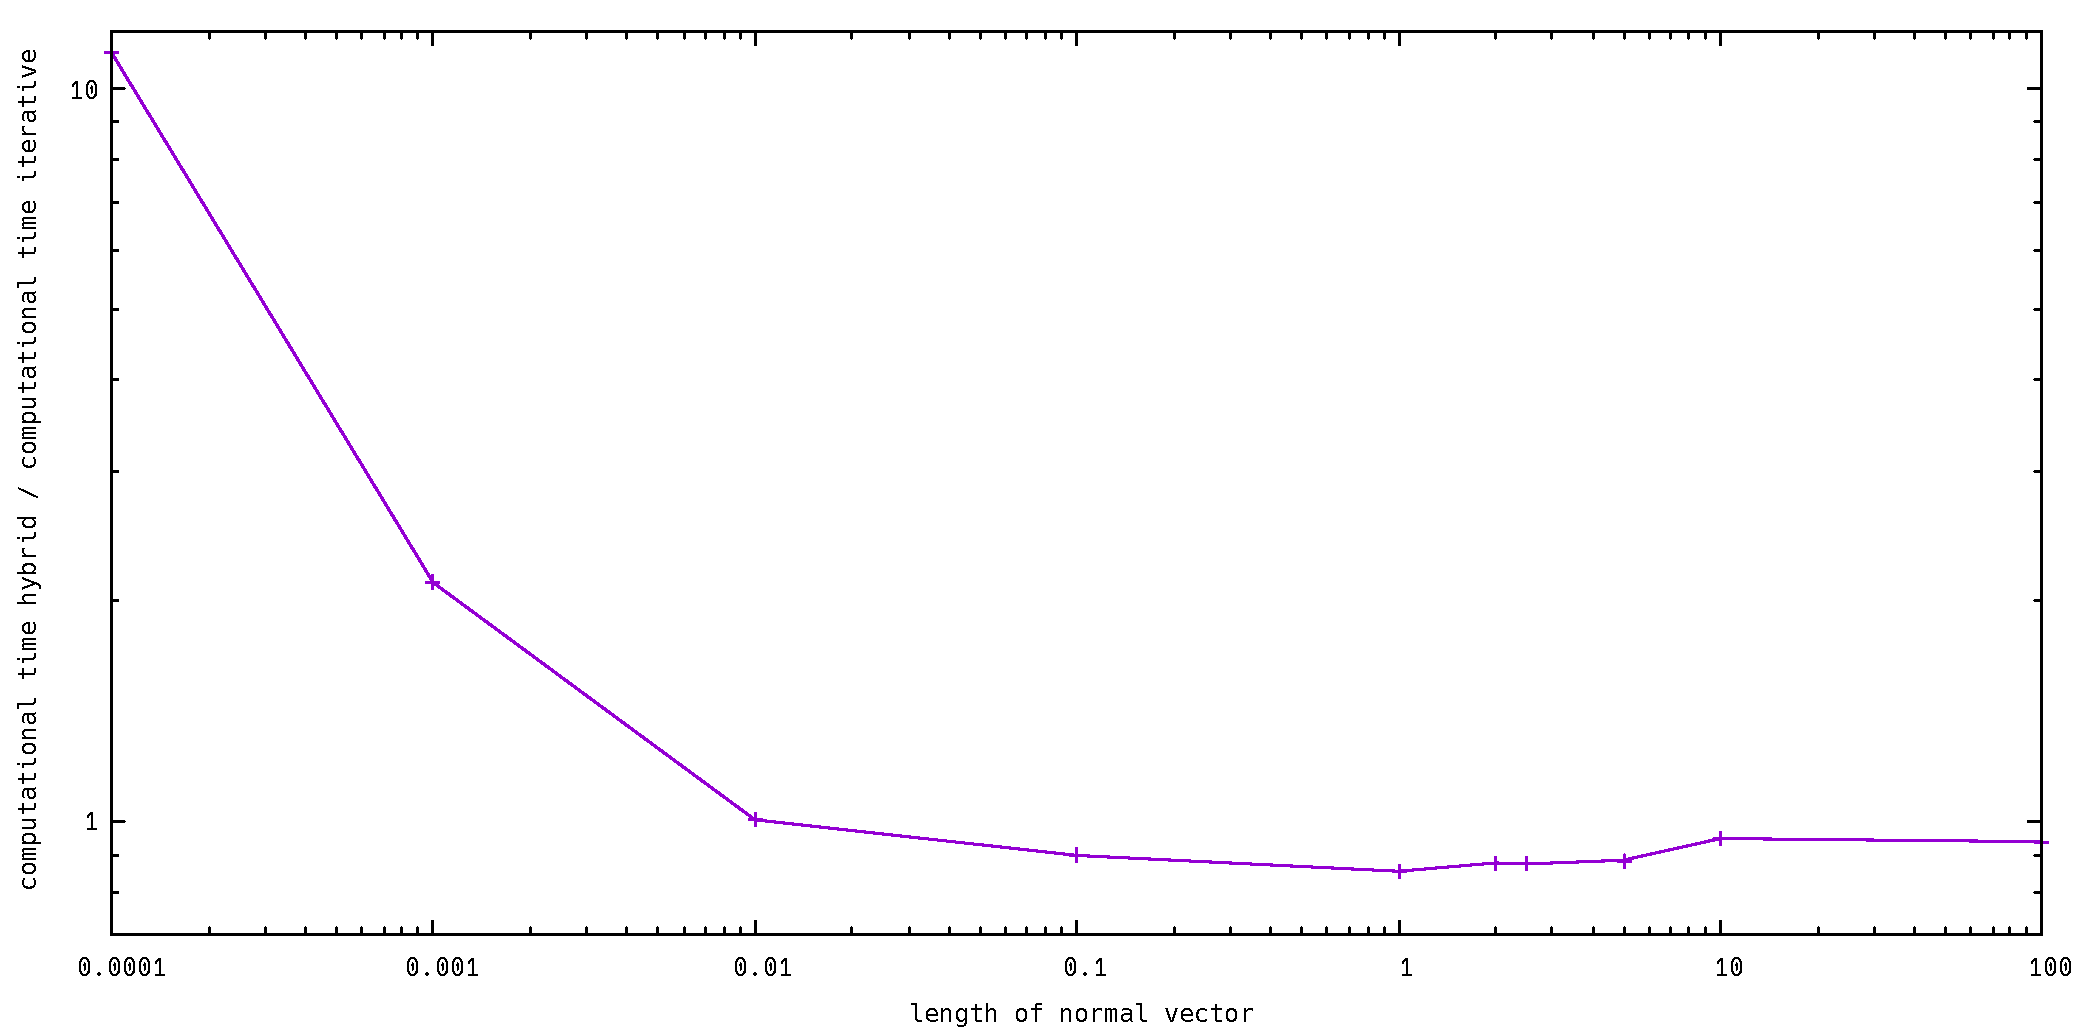
\includegraphics[width=0.8\textwidth]{figures/NormVsTime.pdf}
	\end{minipage}
	\begin{minipage}{\textwidth}
		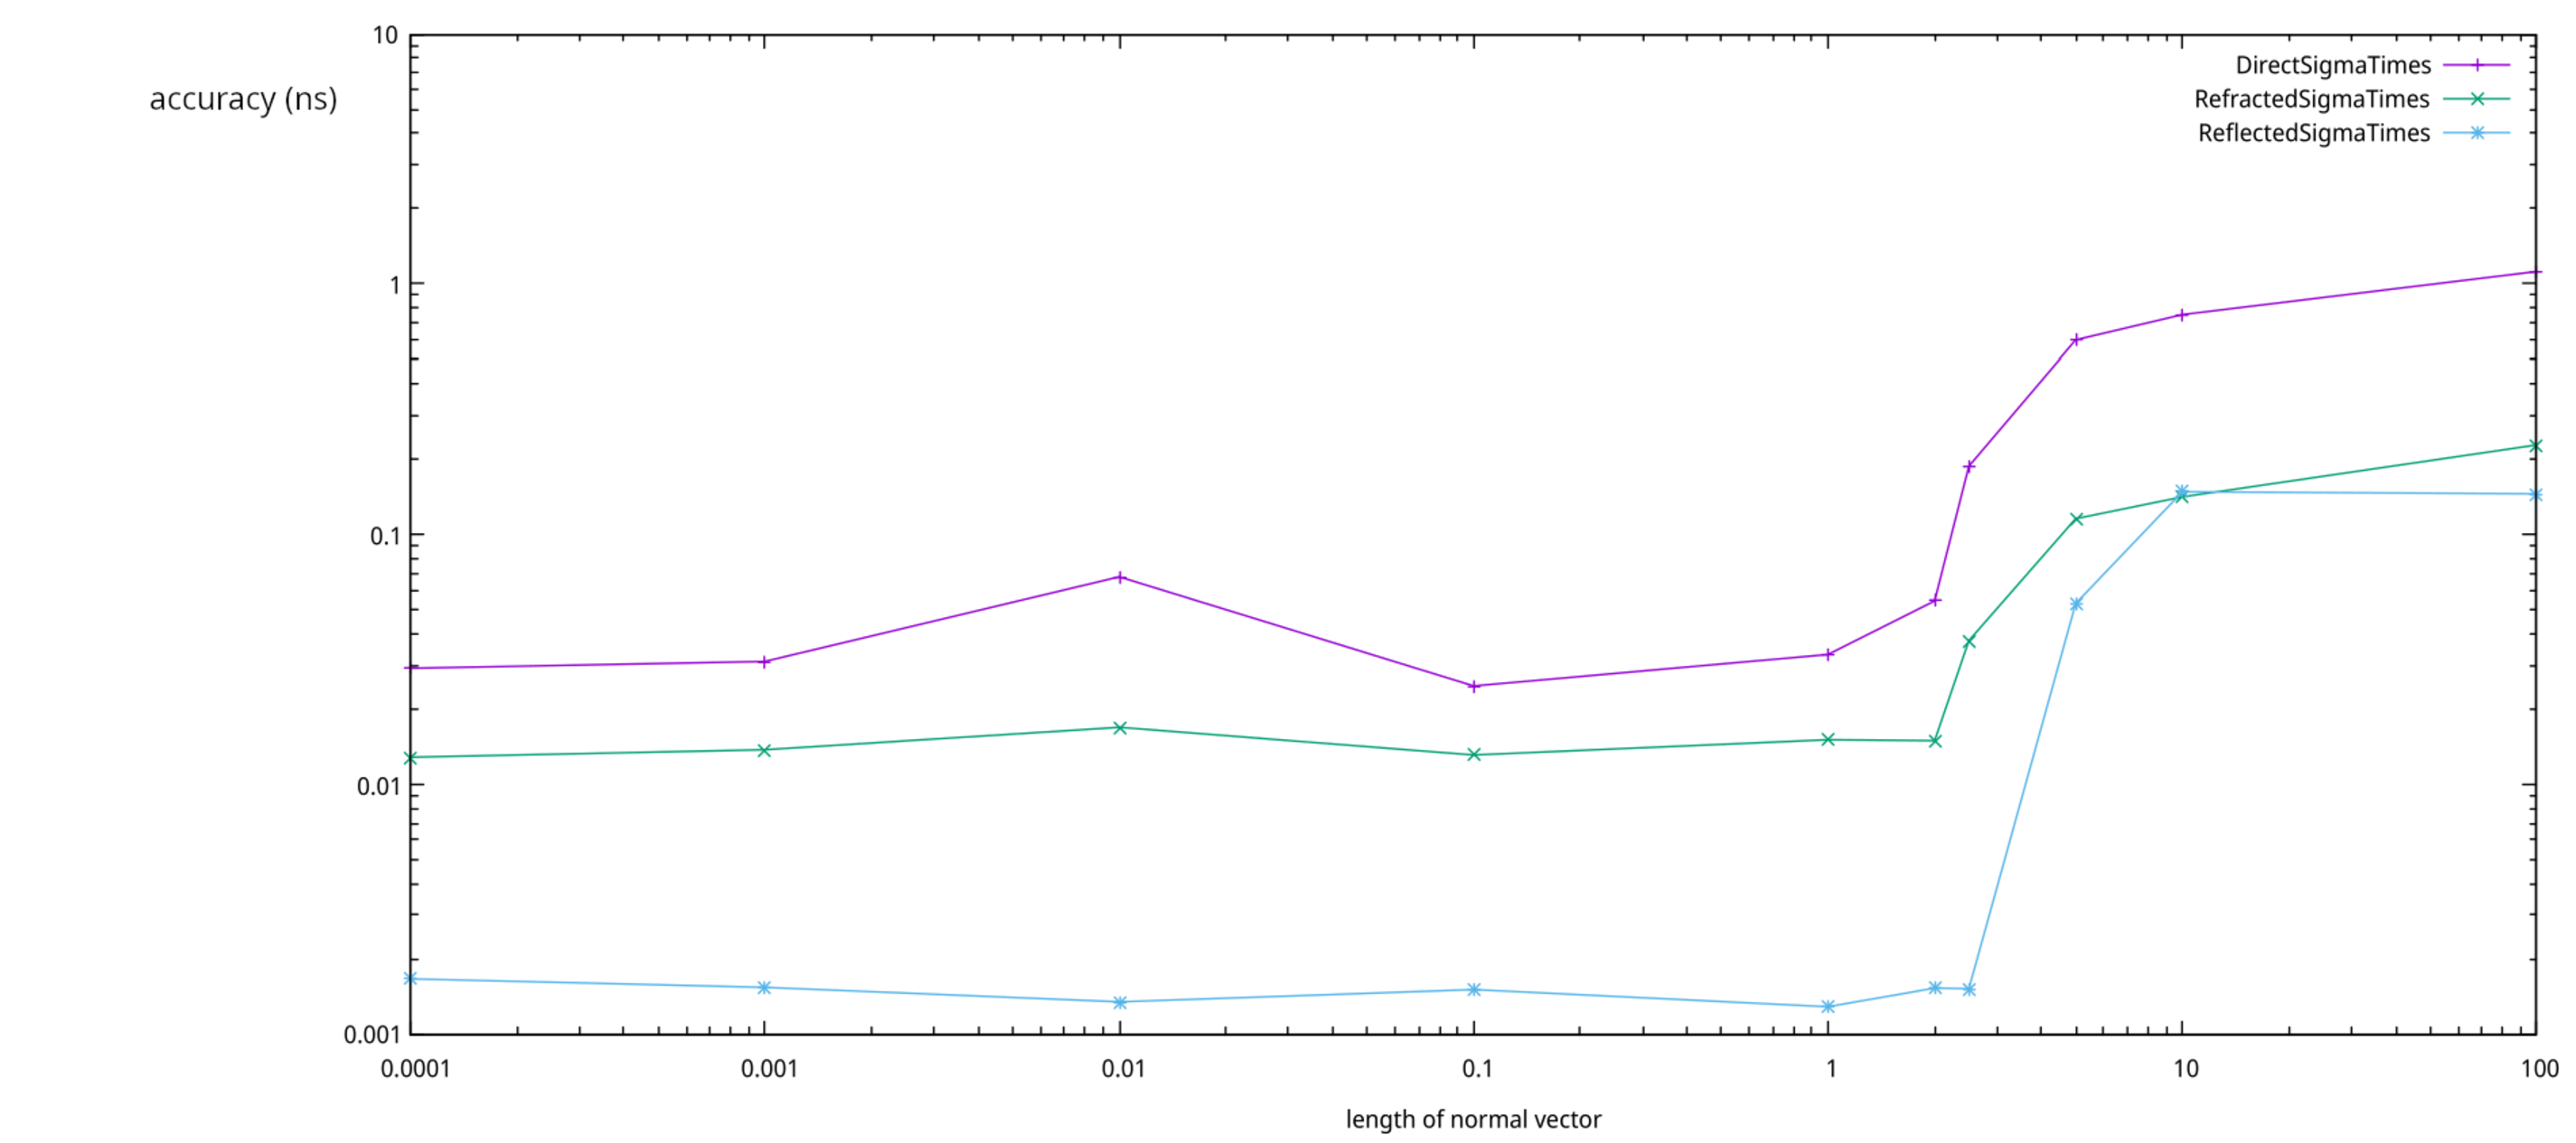
\includegraphics[width=0.8\textwidth]{figures/NormVsSigmaTime.pdf}
	\end{minipage}
\caption{influence of the length of the normal vector}
\label{fig:norminfl}
\end{figure}
\begin{figure}
	\centering
	\begin{minipage}{\textwidth}
		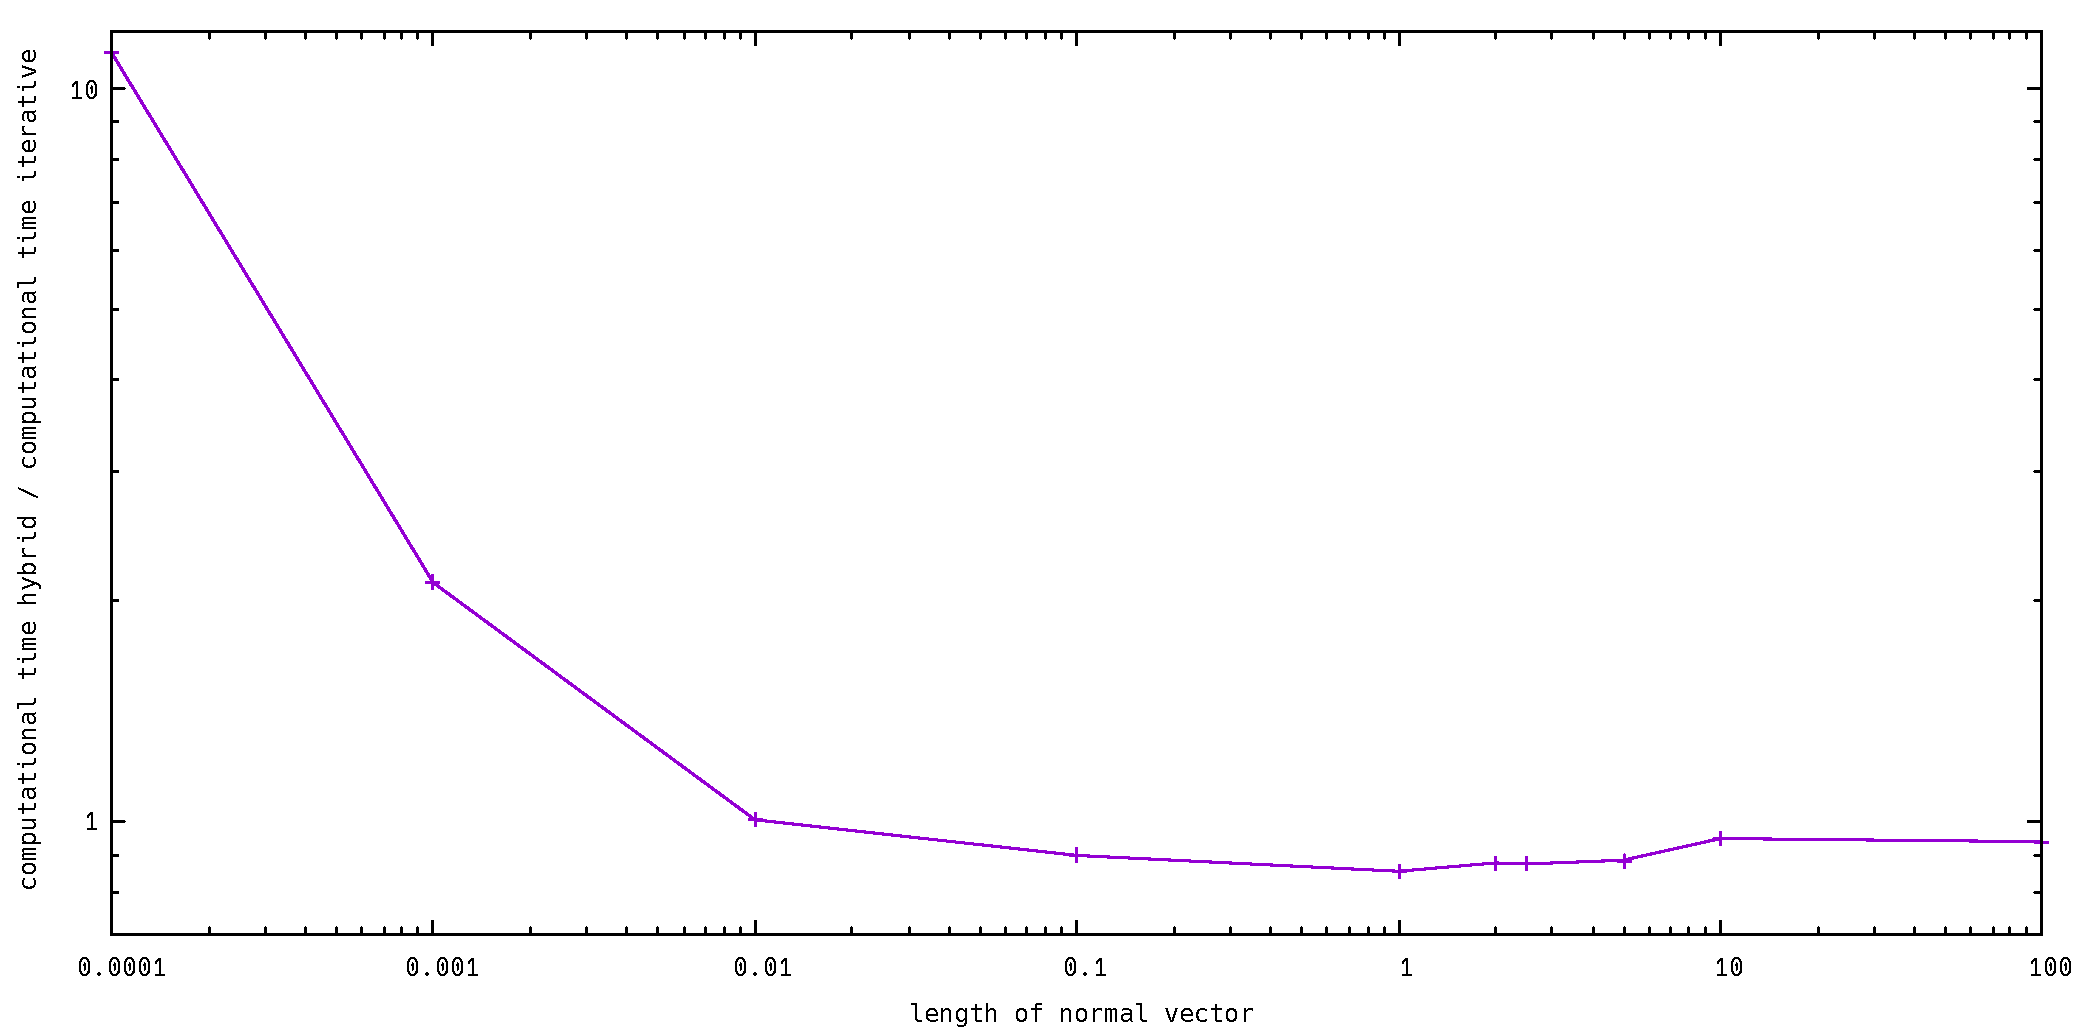
\includegraphics[width=0.8\textwidth]{figures/NormVsTime.pdf}
	\end{minipage}
	\begin{minipage}{\textwidth}
		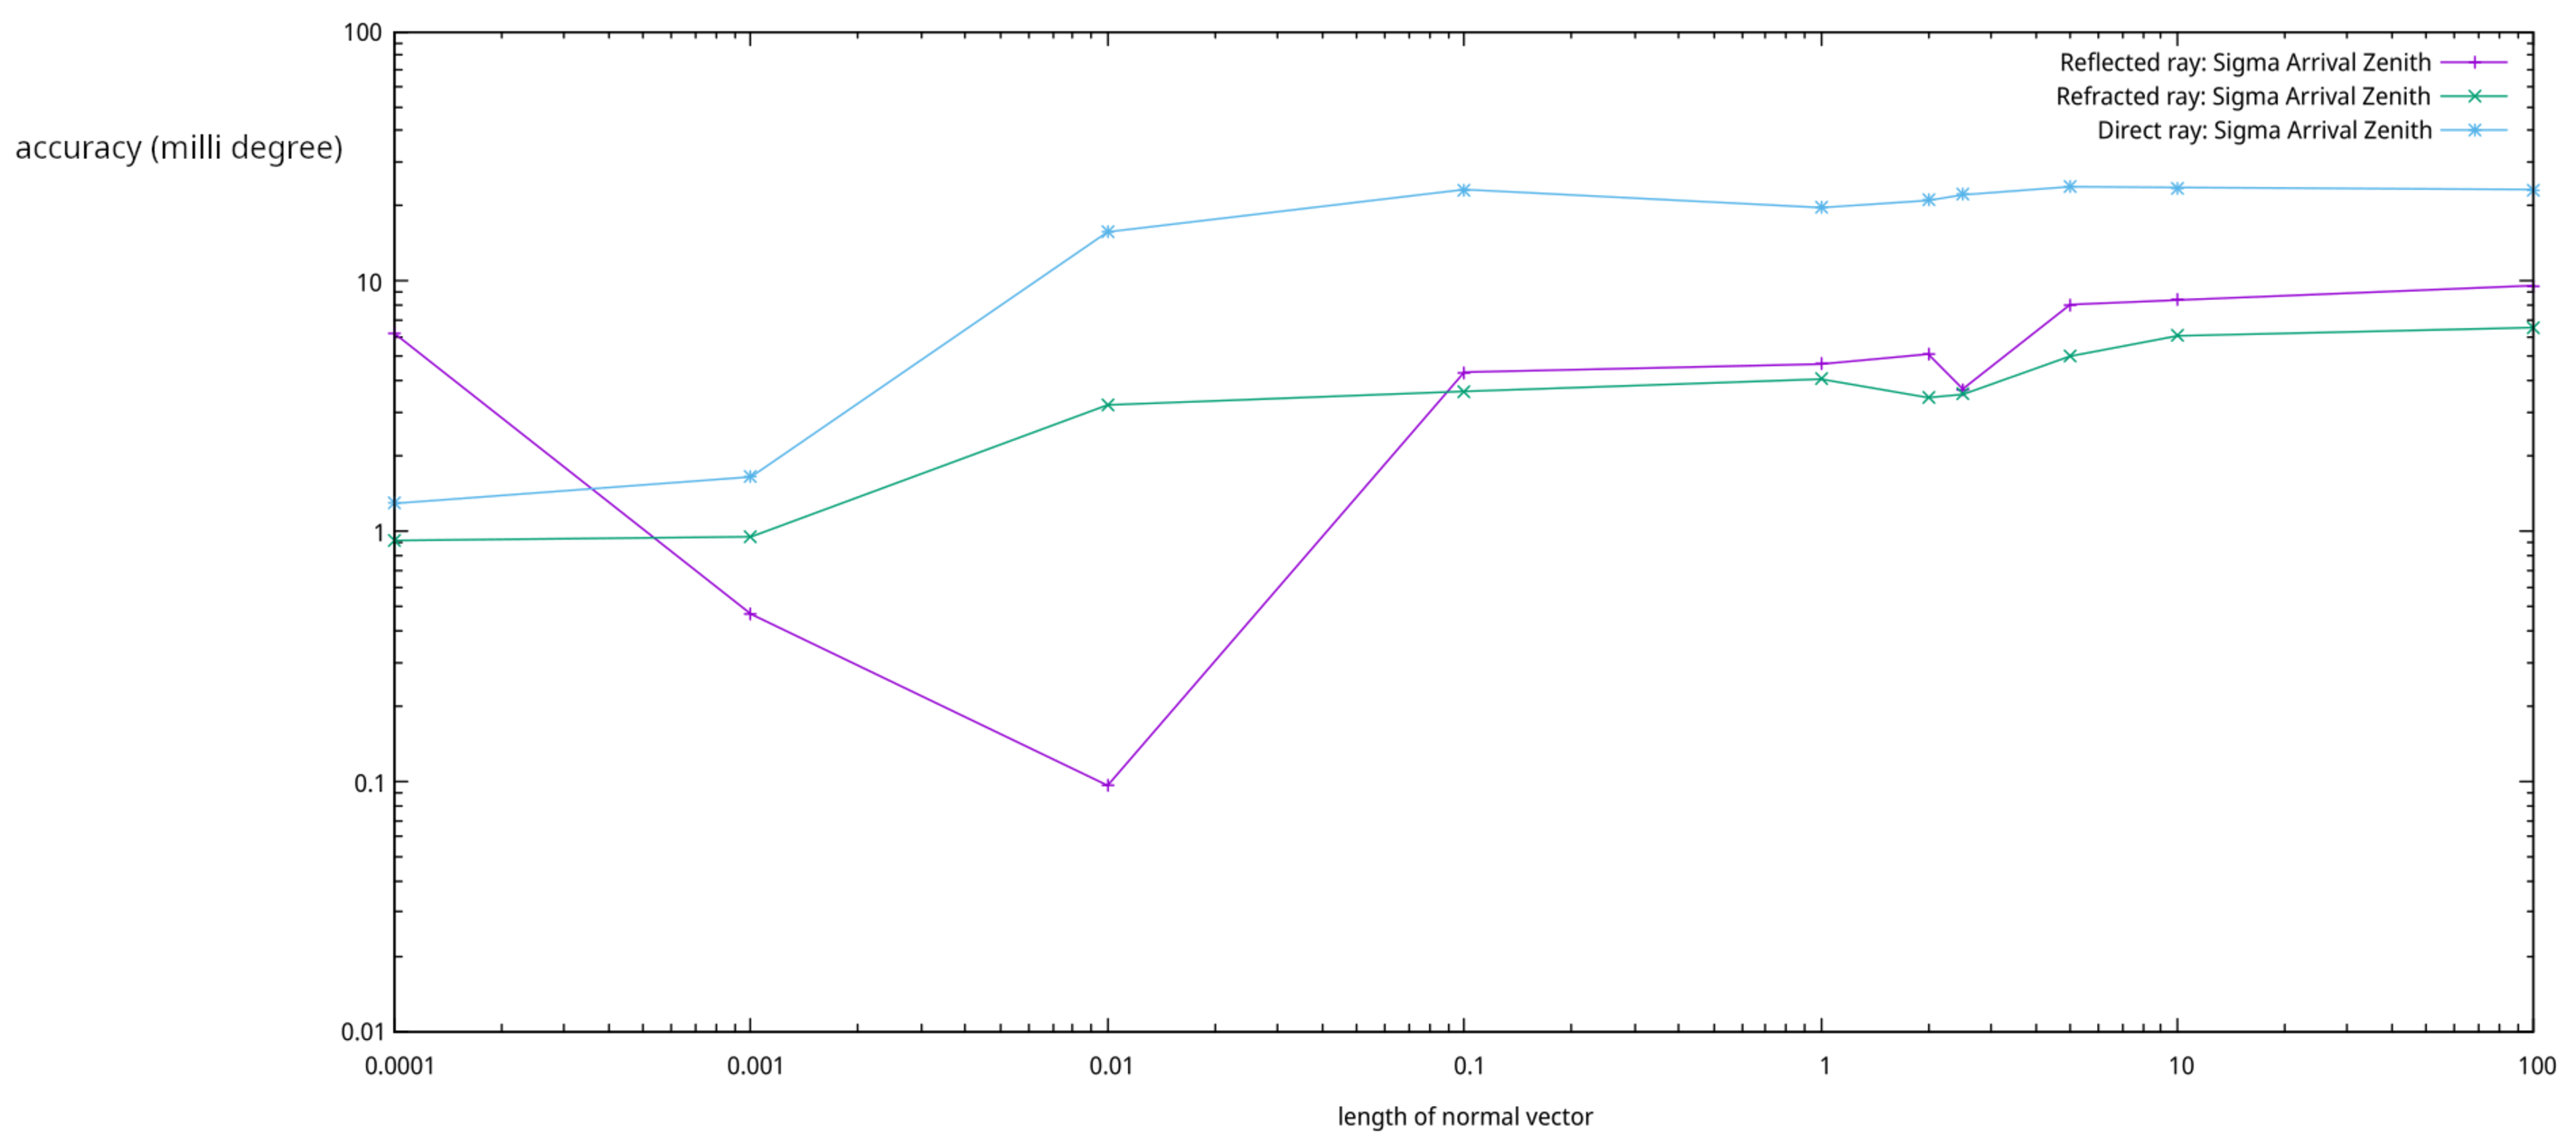
\includegraphics[width=0.8\textwidth]{figures/NormVsSigmaAZ.pdf}
	\end{minipage}
\caption{influence of the length of the normal vector}
\label{fig:norminfl2}
\end{figure}

\subsection{ztol}
We'll now change the \textit{tolerance} on the vertical distance away from the
detector which is deemed accepted i.e in figure \ref{fig:normexpl} if $\Delta
z$ is below this threshold, the minimization procedure is stopped and the last
found answer is the accepted answer.  The results from analogous comparisons as
previously discussed are shown in figures \ref{fig:ztolinfl} and
\ref{fig:ztolinfl2}.  There seems to be a minimum at 0.05m, looking at the
accuracy for this tolerance it seems sufficient to be used.  We can thus infer
the second optimization conclusion: take ztol to be 0.05 m.
\begin{figure}
	\centering
	\begin{minipage}{\textwidth}
		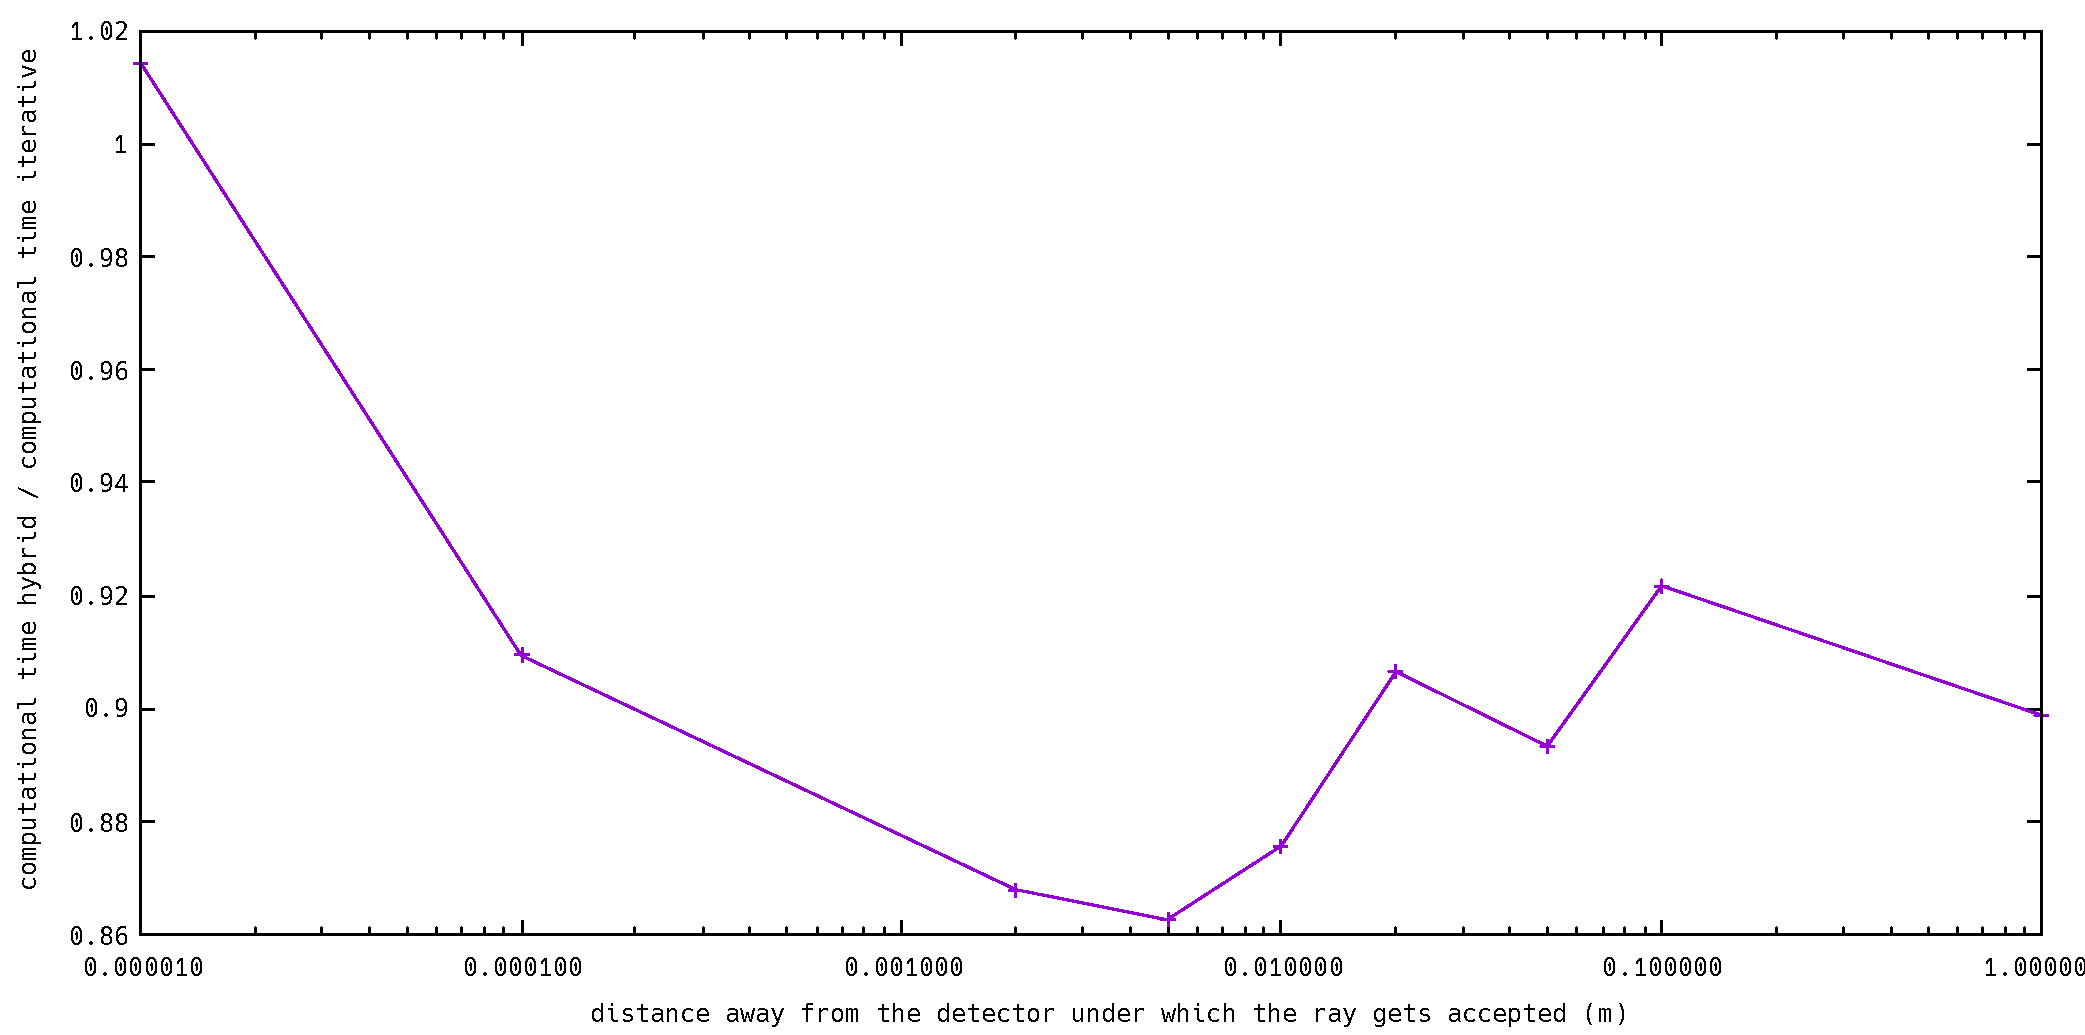
\includegraphics[width=0.8\textwidth]{figures/ZtolVsTime2.pdf}
	\end{minipage}
	\begin{minipage}{\textwidth}
		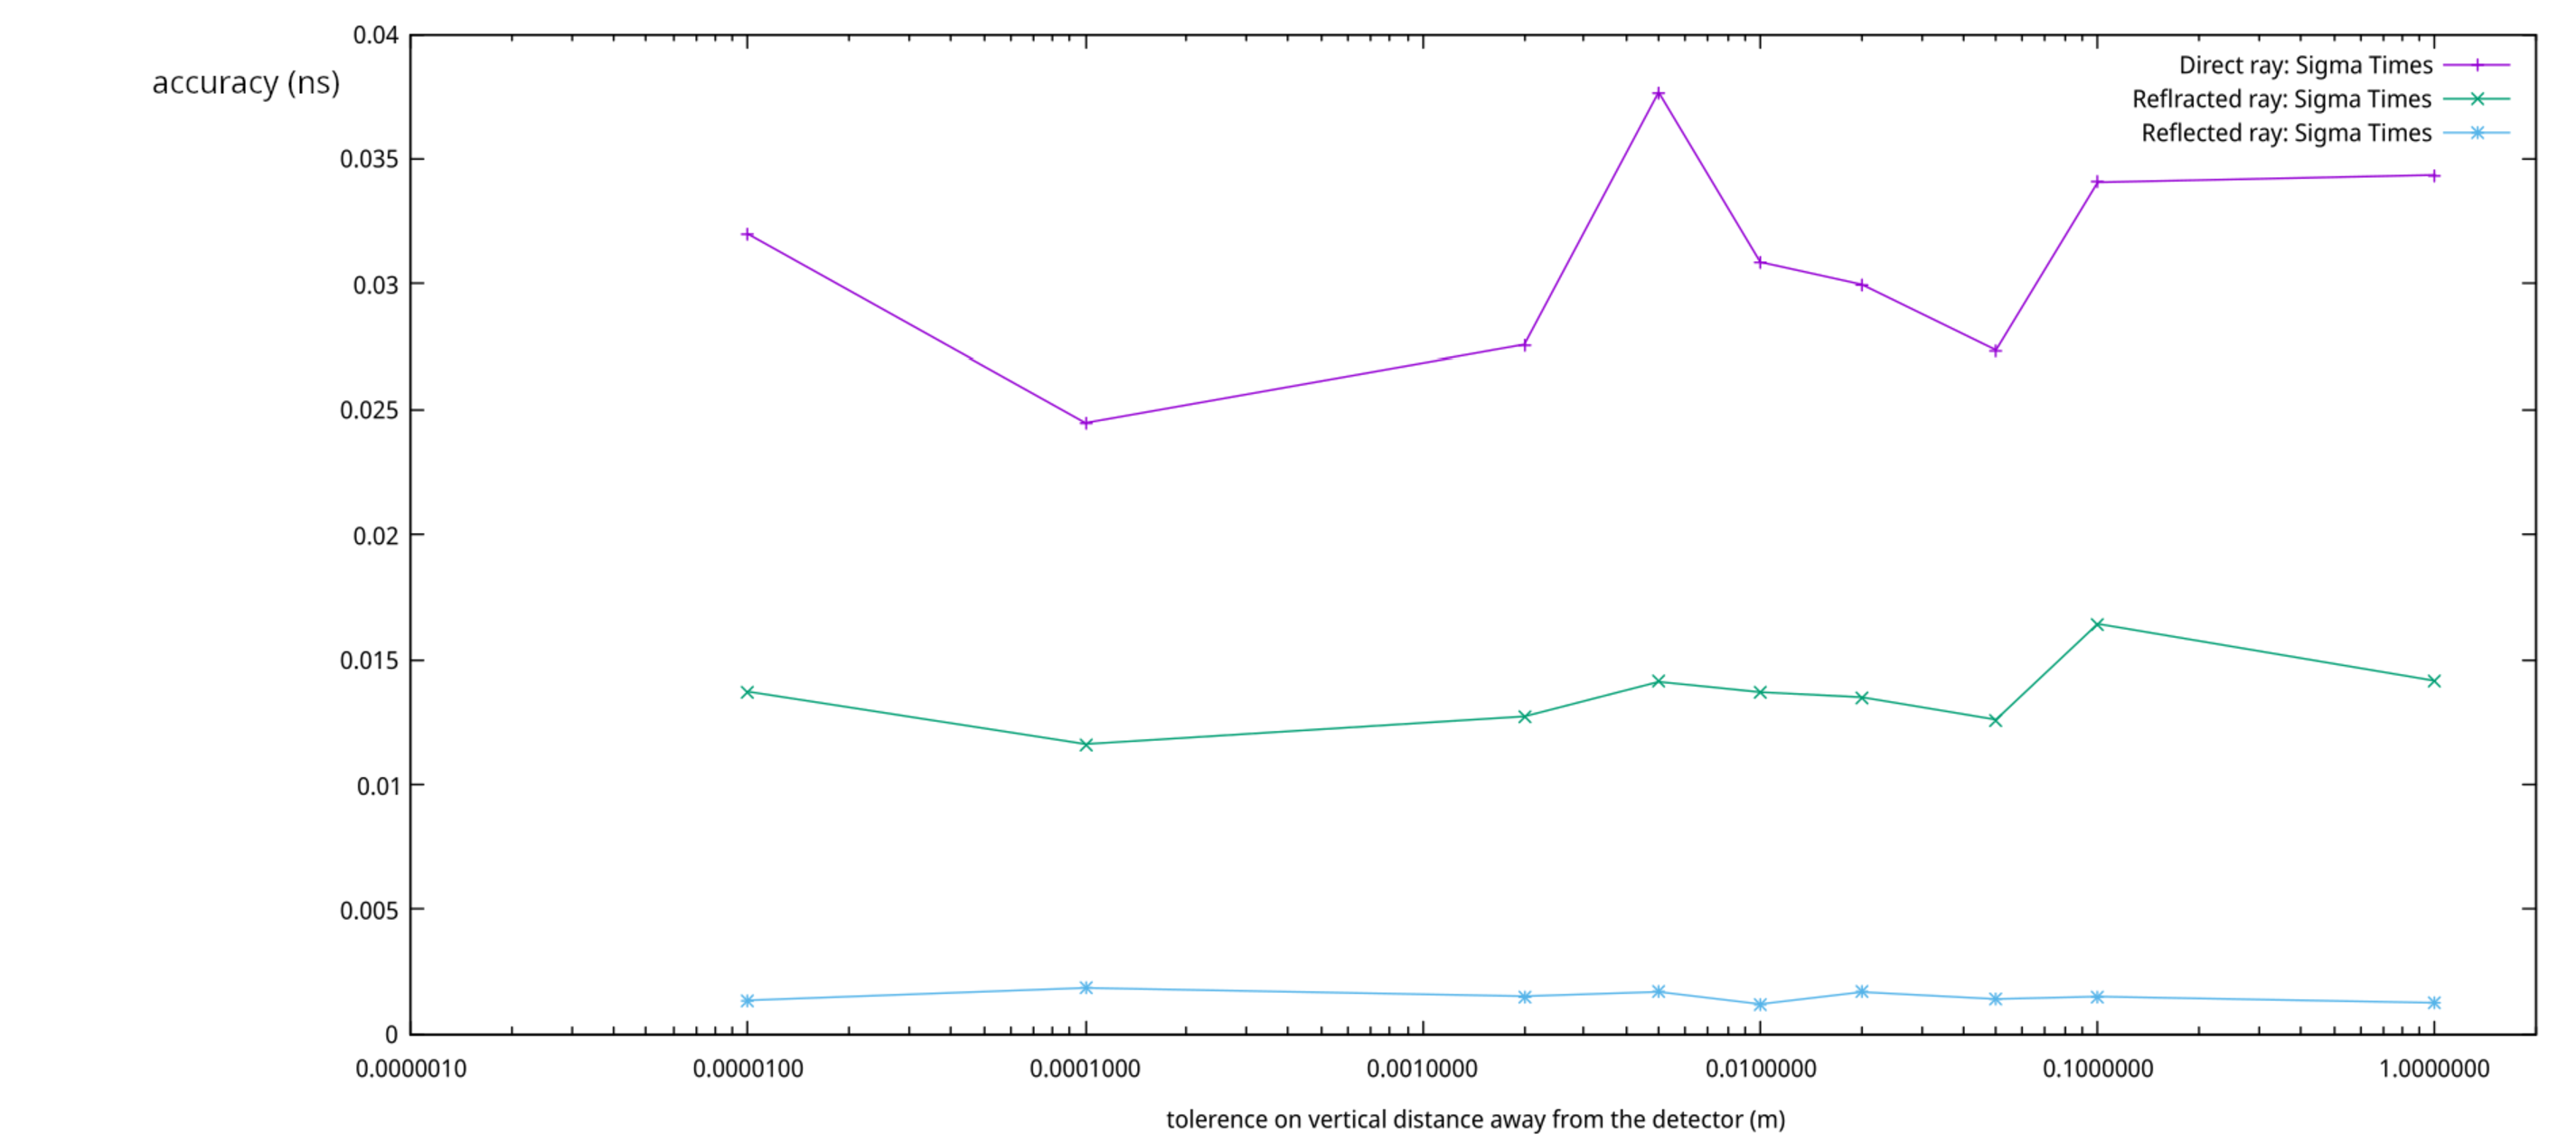
\includegraphics[width=0.8\textwidth]{figures/ZtolVsSigmaTime.pdf}
	\end{minipage}
\caption{influence of the tolerence on vertical distance}
\label{fig:ztolinfl}
\end{figure}

\begin{figure}
	\centering
	\begin{minipage}{\textwidth}
		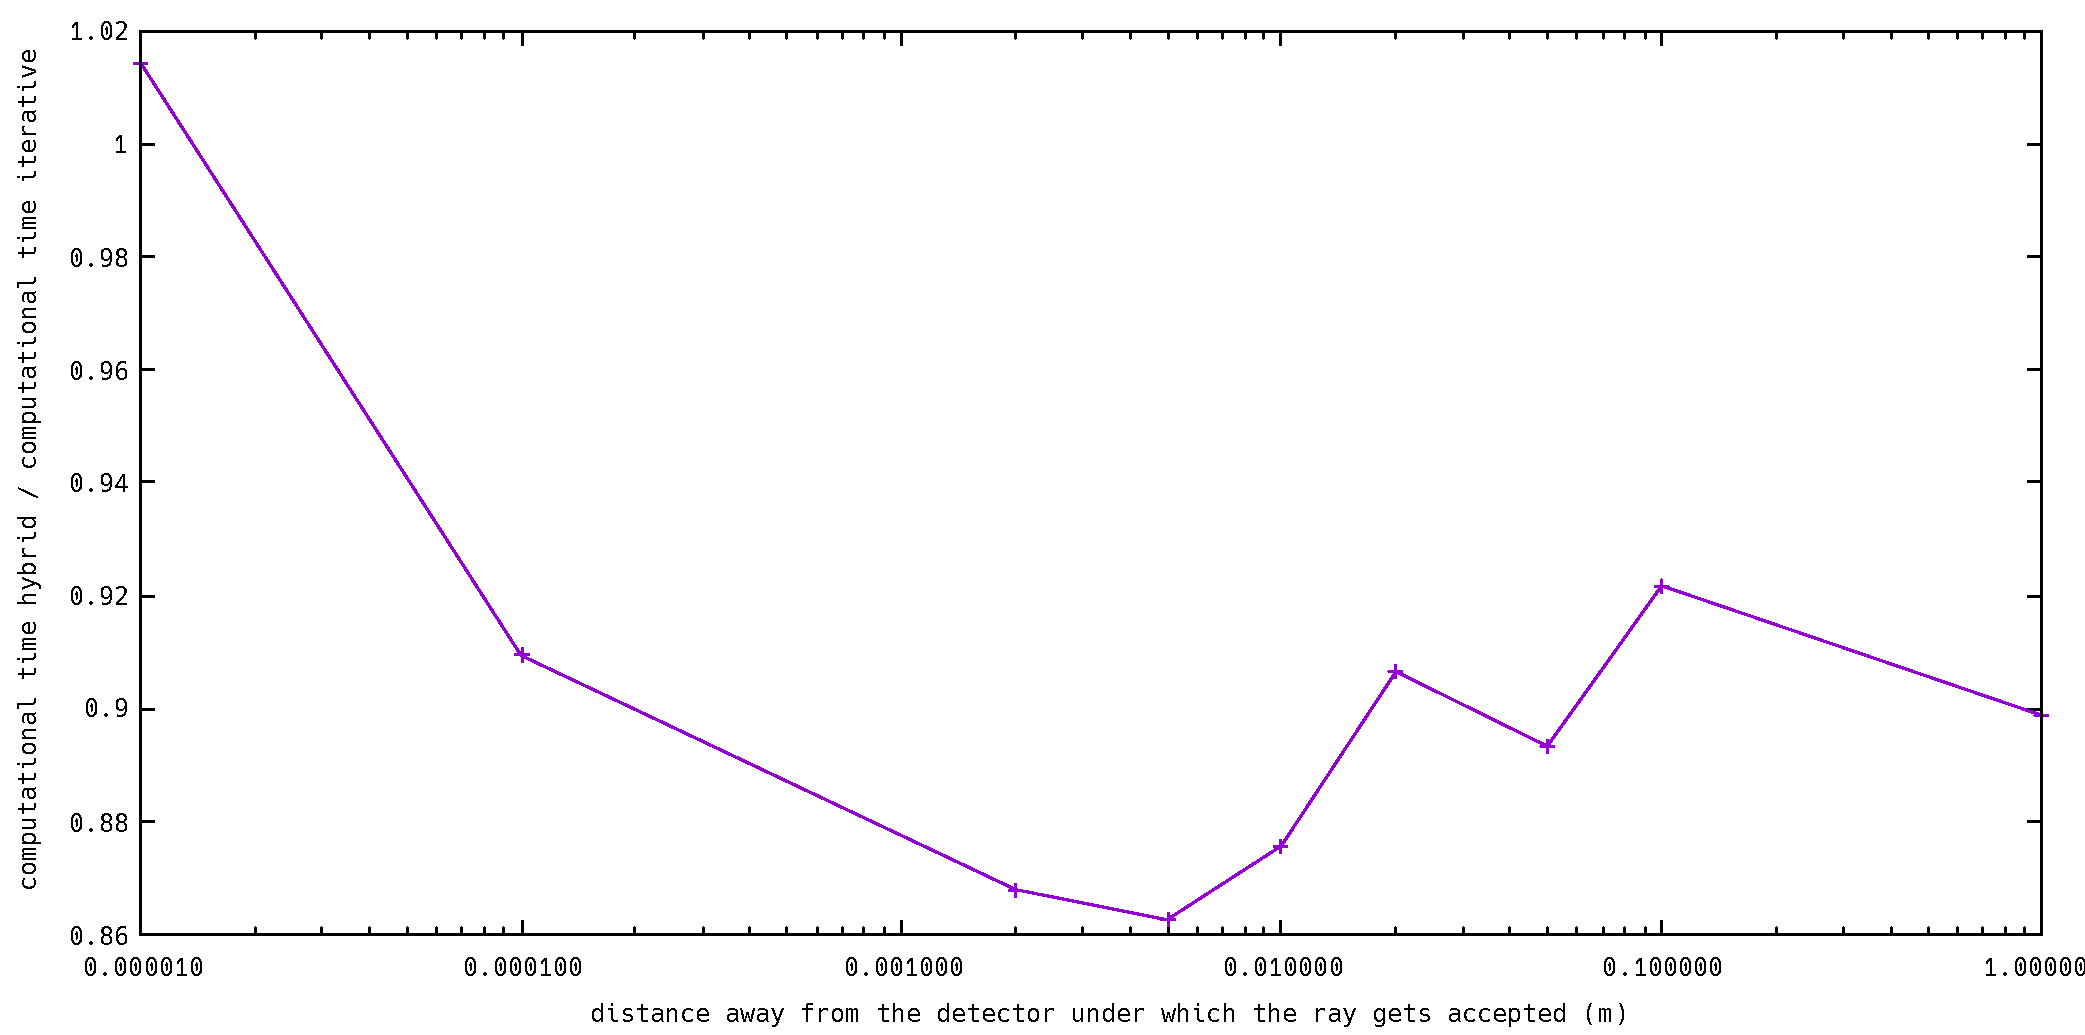
\includegraphics[width=0.8\textwidth]{figures/ZtolVsTime2.pdf}
	\end{minipage}
	\begin{minipage}{\textwidth}
		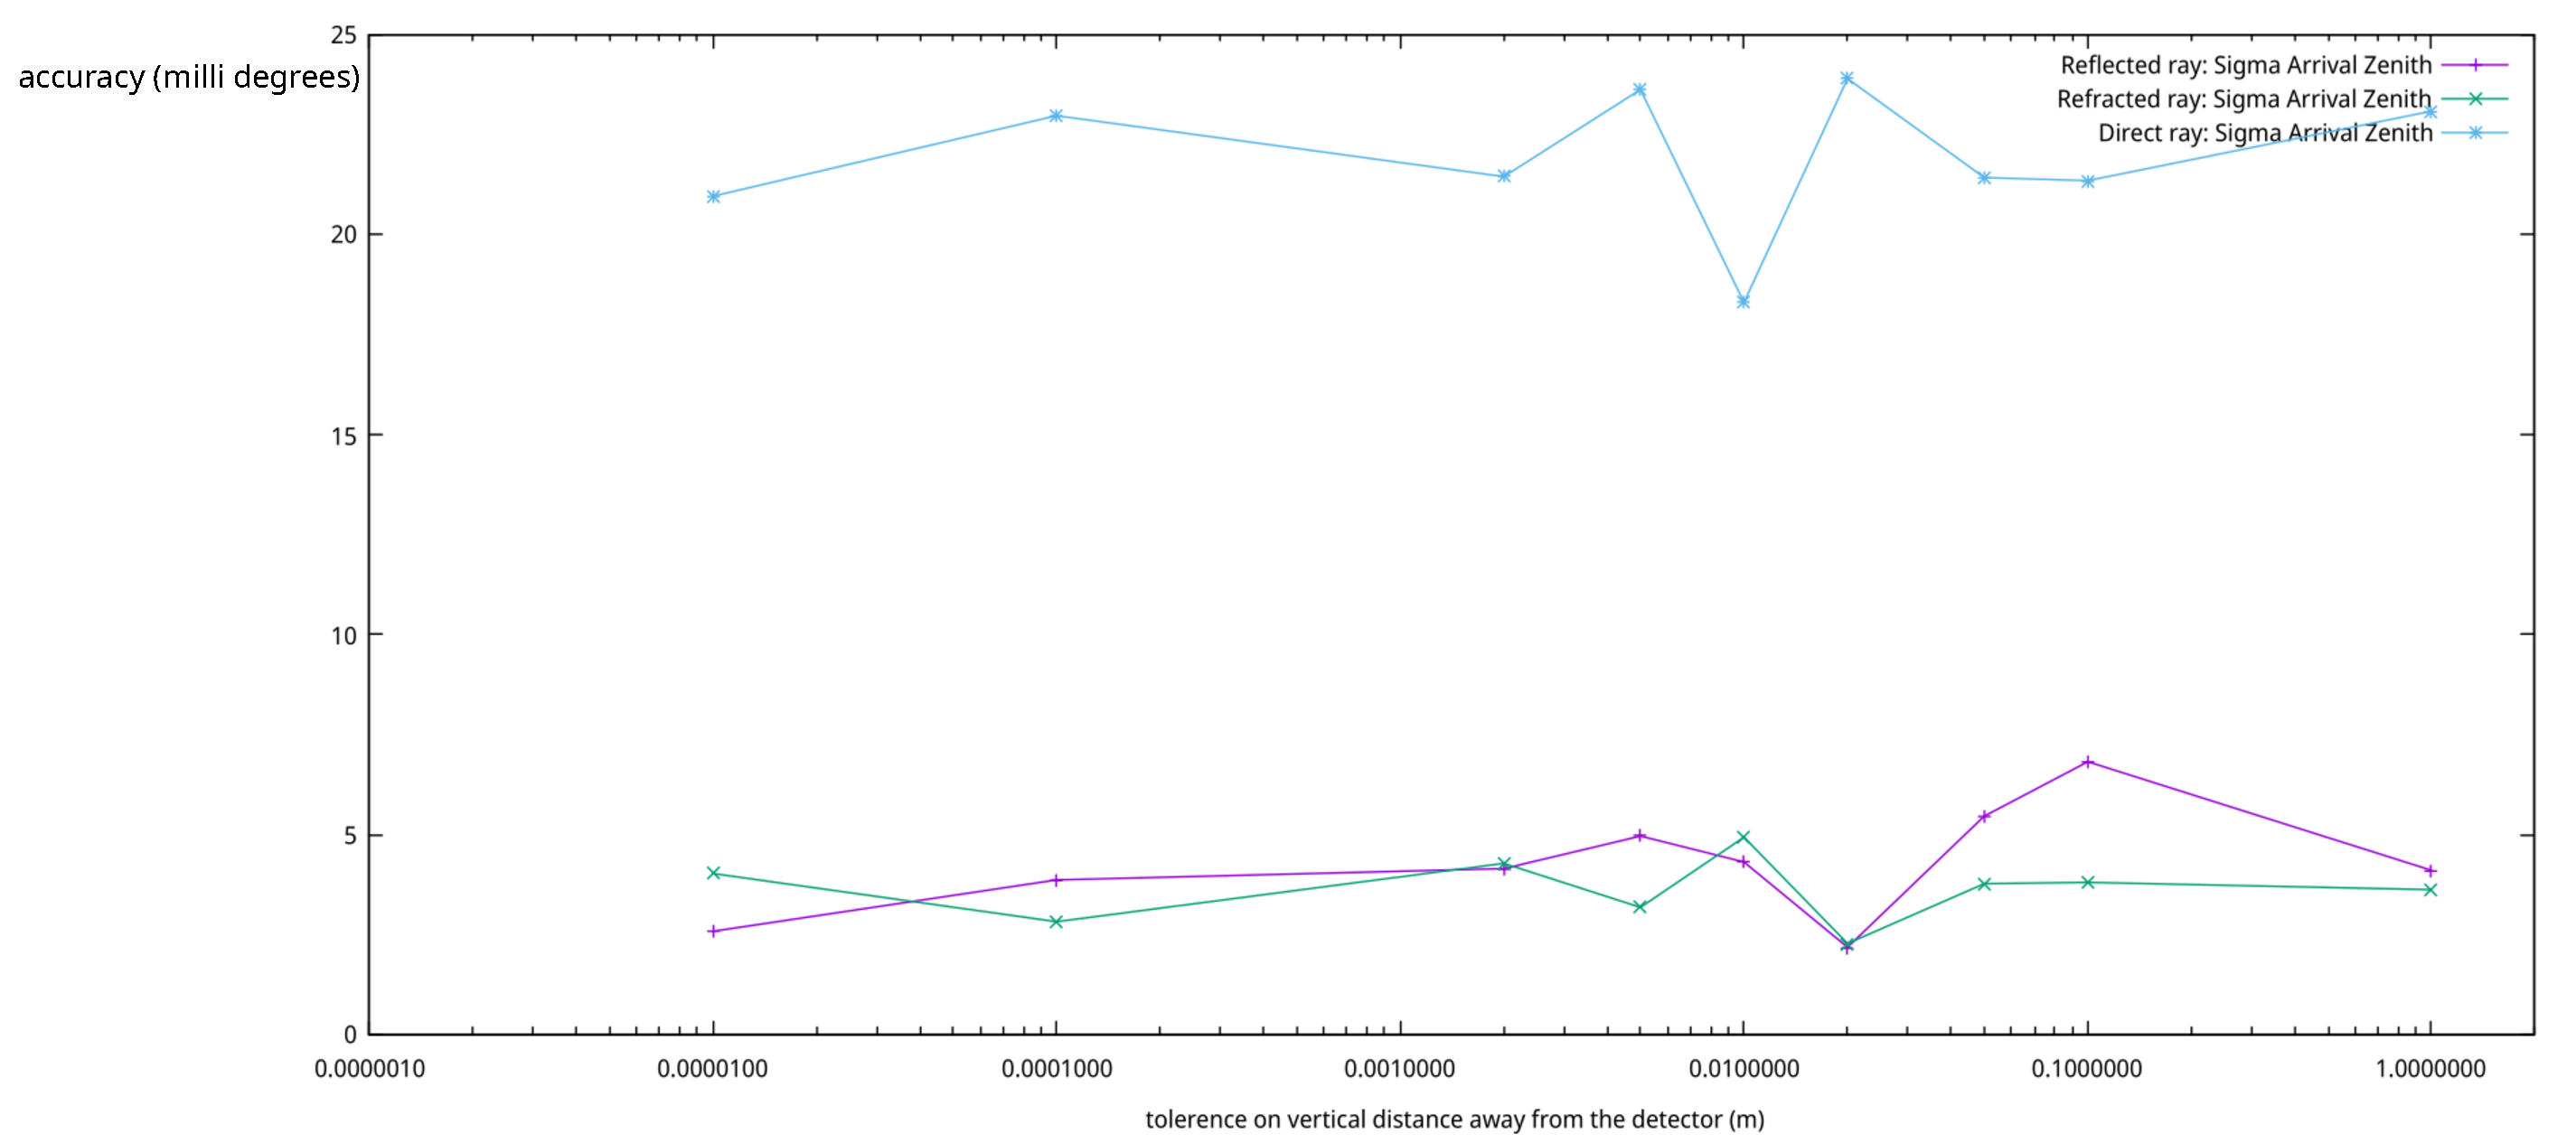
\includegraphics[width=0.8\textwidth]{figures/ZtolVsSigmaAZ.pdf}
	\end{minipage}
\caption{influence of the tolerence on vertical distance}
\label{fig:ztolinfl2}
\end{figure}

\subsection{Sphere Size \& Step Size}
The initial rays are sent out in steps of a certain angle and with a sphere
around the detector of a certain size, varying the parameters of this first
step of the algorithm (e.g the step size and sphere size) might thus have an
effect on both the accuracy and the computational time.  As this initial search
for launch angle regions is also the slowest step in the hybrid ray tracer it's
also the most important step to optimize. The optimization procedure is as
follows: change the sphere size and loop over various step sizes, recording the
speed. Note that, as we have to vary 2 parameters, we can't really look at
accuracy here. This isn't needed however as we'll see that after finding the
optimal solution the accuracy is still superb, apart from one part where it is
needed: \textbf{if insufficient solutions are found}, as we wish this algorithm
to best the iterative ray tracer, it'll need to at least find as many solutions
as the iterative ray tracer does.  If, for a particular random interaction
vertex location, less solutions are found by the hybrid ray tracer than for the
iterative ray tracer, this parameter choice will be thrown away (and colored
differently).  The results of going through this are shown in figure
\ref{fig:SphereStepInfl}, the points colored red are inusable as previously
discussed.

The lower on the graph the points lie, the better. If we combine all the green points into a single plot
we get what is shown on figure \ref{fig:SphereStepFinal},
zooming in onto the lowest point , we see that an optimal sphere size seems to be at 45m accompanied
by a stepsize of 0.7°.

The programs used in making these plots can be found \href{https://github.com/arthuradriaens-code/projects-mt}{here}
under the folder "testhybrid".
\begin{figure}
	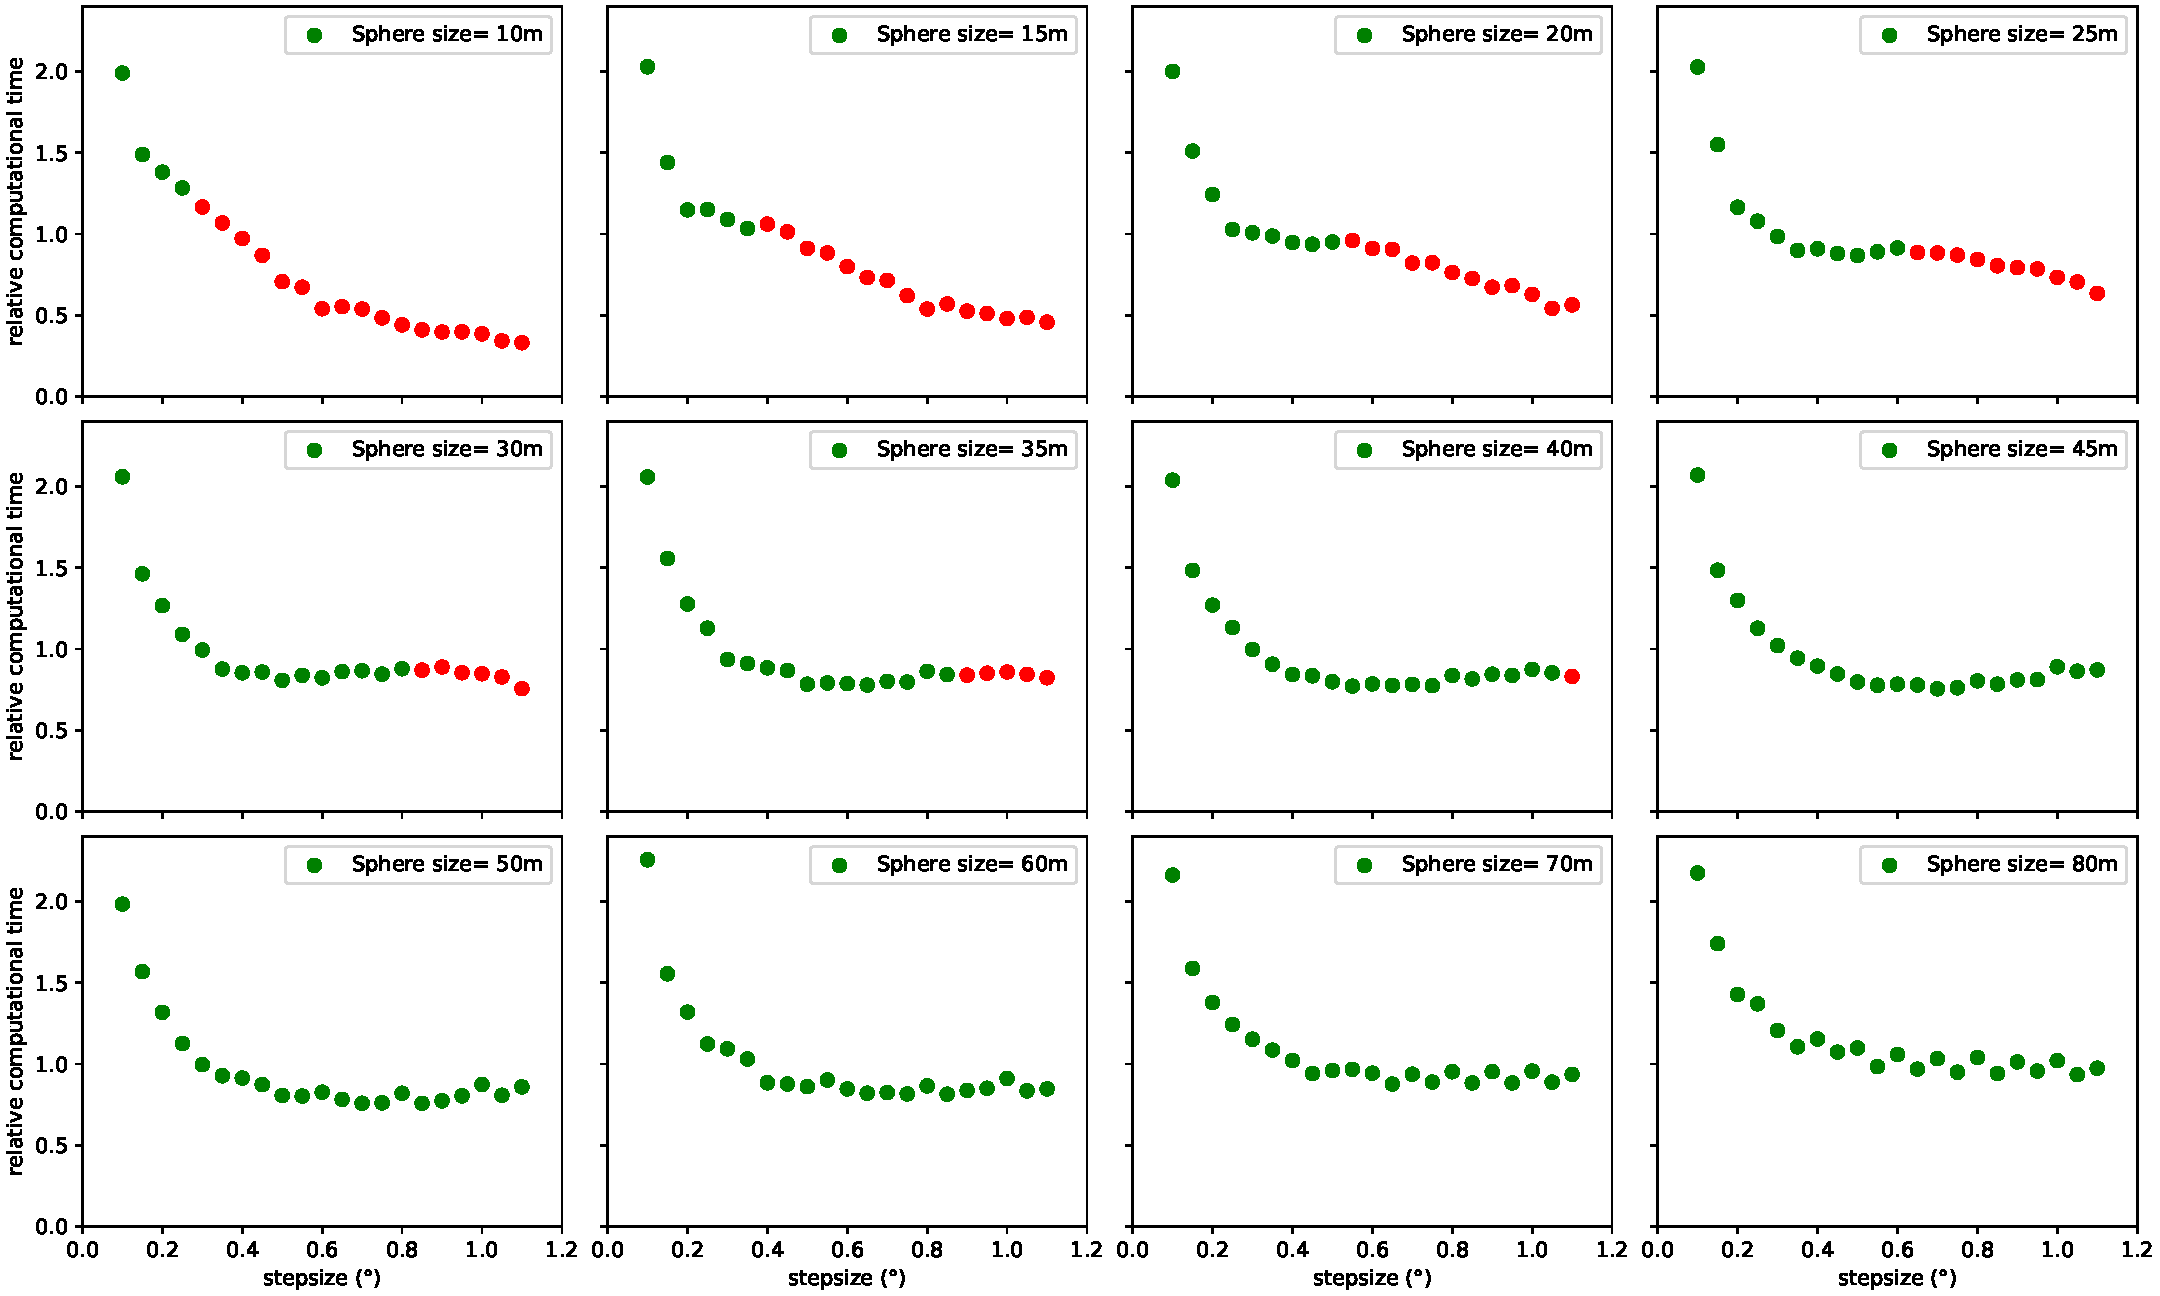
\includegraphics[width=\textwidth]{figures/subplotofallstepsphere.pdf}
	\caption{Variation in Sphere and angle step size with report on relative time.}
	\label{fig:SphereStepInfl}
\end{figure}
\begin{figure}
	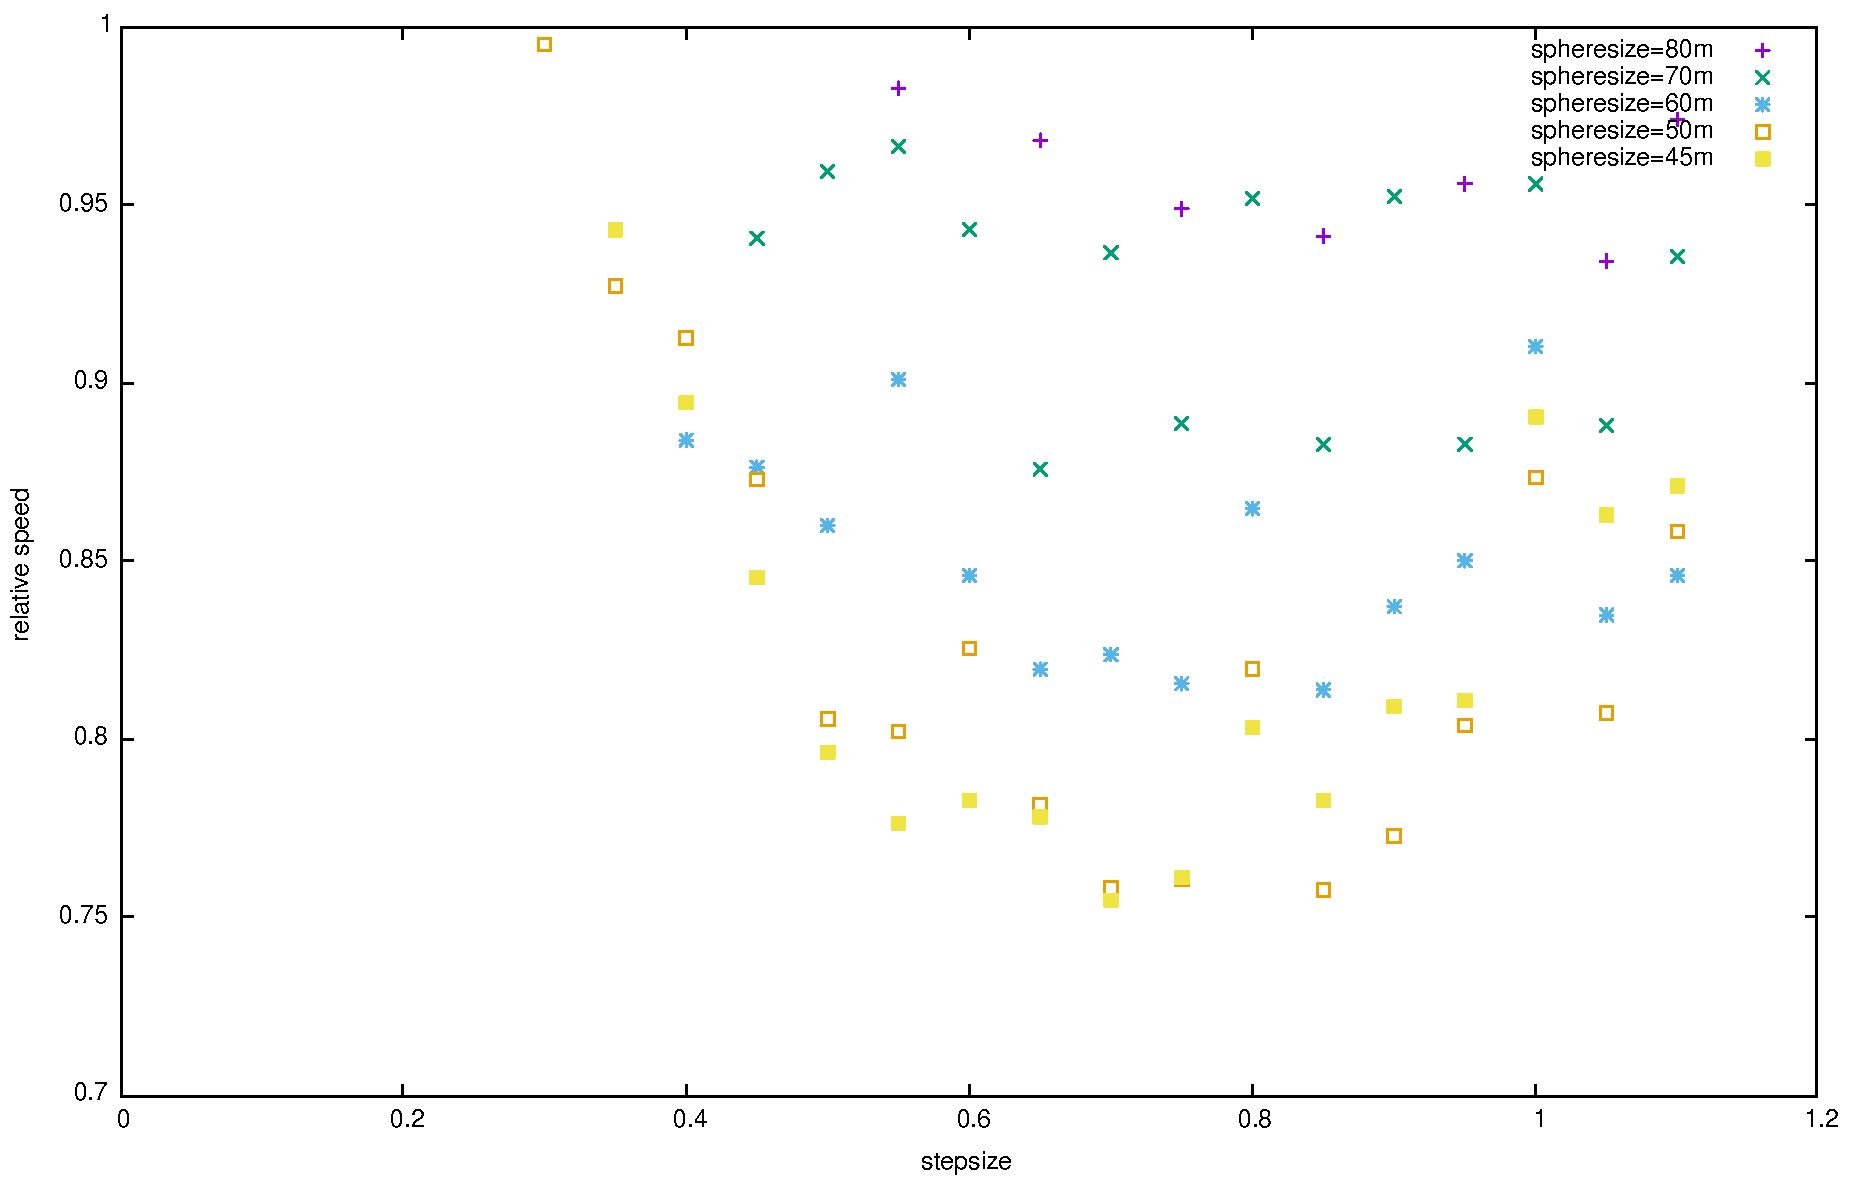
\includegraphics[width=\textwidth]{figures/SphereAndStepFinal.pdf}
	\caption{Green values in variation in sphere and angle step size, max speed (minimum on figure) at 0.7° as stepsize and 45m spheresize}
	\label{fig:SphereStepFinal}
\end{figure}
\newpage
\subsection{Conclusion of optimization}
How does the hybrid ray tracer perform relative to the iterative ray tracer if we use 
the previously optimized variables? After doing a simulation of 1000 random source locations with
the iterative, analytic and hybrid ray tracer and comparing both the iterative to the analytic and the hybrid to the analytic
we get what's shown in figures \ref{fig:acchyb} and \ref{fig:accit}. Where we can clearly see that the hybrid
ray tracer is more accurate, now during this simulation we also recorded the computational speed, the results
are presented below:
\begin{itemize}
	\item iterative: 0.61 computations/s
	\item hybrid: 0.82 computations/s
	\item analytic (c++ compiled version): 10289 computations/s
\end{itemize}
The hybrid ray tracer is thus 33.7\% faster than the iterative ray tracer, the speed of the analytic ray tracer
has a difference of the other two which might seem quite overwhelming but this can get mitigated in the future if 
part of the hybrid ray tracer gets re-written in a compiled language (like c++).

\begin{figure*}
	\centering
\begin{minipage}{0.49\textwidth}
	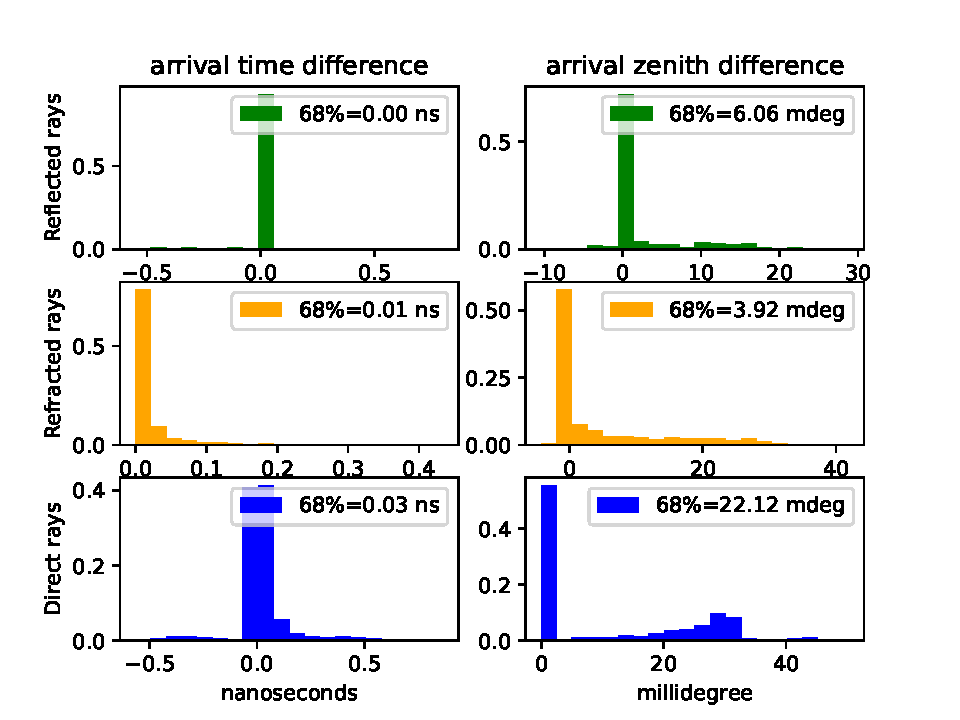
\includegraphics[width=1.1\textwidth]{figures/hybrid_comparison_N_1000.pdf}
	\caption{Hybrid}
	\label{fig:acchyb}
\end{minipage}
\begin{minipage}{0.49\textwidth}
	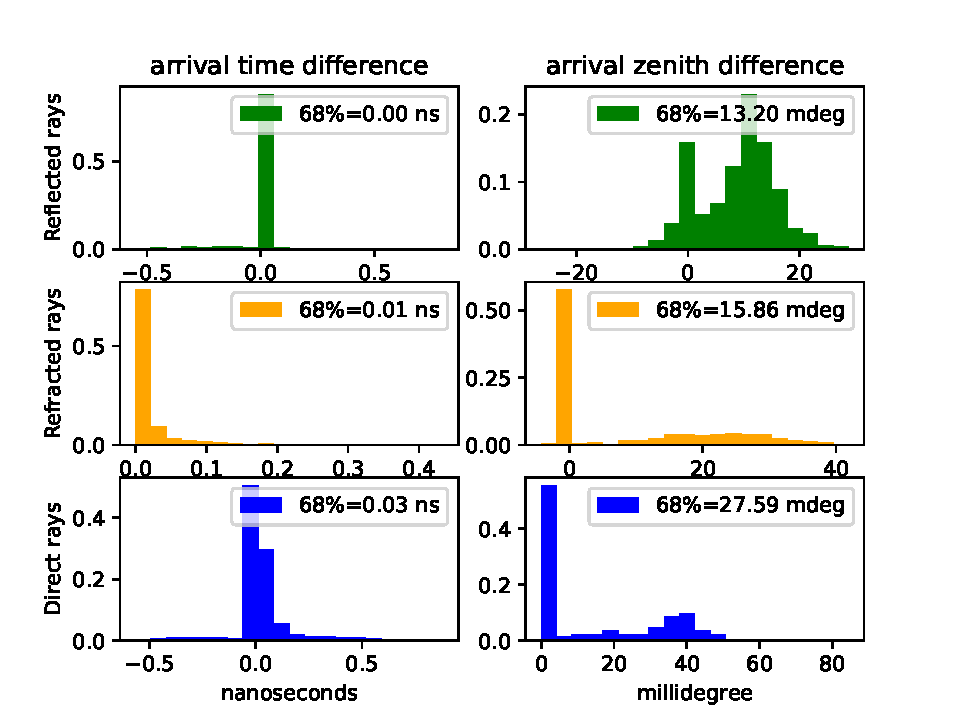
\includegraphics[width=1.1\textwidth]{figures/iterative_comparison_N_1000.pdf}
	\caption{Iterative}
	\label{fig:accit}
\end{minipage}
\end{figure*}

\section{Expansion}
Using the ray tracer as it is now defined makes us unable to calculate paths by
\textit{secondaries}.  When your ice model has some kind of added complexity
like a reflective bottom or a discontinuity layer (like what will be the case
for our air-bourne balloon in the next chapter) you'll need to account for
secondaries, these are additional rays like an extra refracted or reflected
rays that get generated at this discontinuity. How the algorithm is now it will
follow one ray from the source to the discontinuity and only consider, say, the
reflected ray. Whilst a refracted ray generated at such a discontinuity might
actually end up closer to the detector.

To implement secondaries, we'll just check if there are any found at the
delta\_z algorithm and if so loop over them, keeping the original ray's $\Delta
z$ in mind as the "global best" and looking if any of the secondary rays'
$\Delta z$ is lower than the "global best" if so this will be considered the
new final ray which gets returned and the $\Delta z$ that gets returned is the
new "global best" originating from the secondary. If there is no secondary
ending closer than the "original" ray than the original ray with it's $\Delta
z$ is returned.


